\documentclass[a4paper,pdftex,oneside,10pt,mathsans]{scrartcl} %,fleqn

% Wir geben alles im UTF-8 Zeichensatz ein (alles andere ist Unfug!)
\usepackage[T1]{fontenc}
\usepackage[utf8]{inputenc}
\usepackage{ngerman}

\newcommand{\Autoren}{\href{buchegger.uni@gmail.com}{Philipp Buchegger}}

\newcommand{\Gruppe}{Studenarbeit}
\newcommand{\Thema}{Disks}
\newcommand{\Titel}{Binärsternsysteme}
\newcommand{\Datum}{Tübingen, den \today}
\newcommand{\Schluesselwoerter}{}


\usepackage{ae}

% Wir verwenden die neue deutsche Rechtschreibung (wir versuchen es zumindest ^^)
\usepackage{ngerman}
\usepackage[english,ngerman]{babel}

% Wir m�hten Grafiken verwenden und diese sollen als Ausgabetreiber pdfTex verwenden
\usepackage[pdftex]{graphicx}

% Keine Papierverschwendung wie es bei Tex-Standard blich ist
\usepackage[bottom=30mm,top=25mm,inner=20mm,outer=20mm,marginparwidth=15mm,marginparsep=3mm,headsep=10mm]{geometry}

% Die zus�zlichen AMS-Mathepakete, und sch�ere Integralgrenzen
\usepackage[intlimits]{amsmath}
\usepackage{amsthm}
\usepackage{amsopn}
\usepackage{amscd}
\usepackage{amsfonts}
\usepackage{amssymb}
%\usepackage{mathrsfs}

% Einheitenbefehle \unit und \unitfrac
\usepackage{units}

% Sch�ere und flexiblere Kopfzeilen
\usepackage{fancyhdr}

% Ab und zu m�hten wir Seiten im Querformat einbauen
\usepackage{pdflscape}

% Vorschau PDFs erstellen
\usepackage{thumbpdf}

% Type1-Fonts (damit die PDFs nicht so verpixeln)
% Folgende Pakete sollten deshalb installiert sein:
% Font-Packages: CTAN: fonts/cmbright/, CTAN: fonts/ps-type1/cm-super/, CTAN: fonts/ps-type1/hfbright/
\usepackage{type1cm}

% Komplette PDFs (oder Seiten daraus) importieren
\usepackage{pdfpages}

% If-Abfragen erm�lichen
\usepackage{ifthen}

% Quellcodes sch� darstellen
\usepackage{verbatim}

% Erweitere Quellcodedarstellung
\usepackage{listings}

% Verschiedene Pakete (was machten die nochmals?)
\usepackage{titling}
\usepackage{textcomp}
\usepackage{nonfloat}
\usepackage{booktabs}

% Erweitere Aufz�lungen
\usepackage{eqlist}
\usepackage{paralist}

% Farbuntersttzung
\usepackage{color}

% PDF spezifische Funktionen
\usepackage[a4paper,breaklinks,unicode,colorlinks,linktocpage,pdftex,linkcolor=blue,urlcolor=blue,backref,pagebackref,bookmarks,bookmarksnumbered]{hyperref}

% dsfont
\usepackage{multicol,wasysym,expdlist}

% kleine Layoutfehler fixen
\usepackage{ellipsis,fixltx2e,mparhack}

\usepackage{microtype}

% absolute Textpositionierung
\usepackage{textpos}

% Indexerstellung
\usepackage{makeidx}
\usepackage{booktabs}

% Immer Serifenlos schreiben
\renewcommand{\familydefault}{\sfdefault}

% Abs�ze nicht einrcken
\setlength{\parindent}{0em}

% Titel, Autor, Datum konfigurieren (fr Titelseite)
\title{ \textbf{\Titel} \\ \Thema}
\ifthenelse{ \equal{\Gruppe}{} }{ \author{\Autoren} }{ \author{\Autoren \\ \Gruppe}}
\date{\Datum}

% PDF Informationen
\hypersetup{
  pdftitle=\Titel,
  pdfsubject=\Thema,
  pdfauthor=\Autoren,
  pdfkeywords=\Schluesselwoerter,
  pdfcreator={LaTeX},
  pdfproducer={LaTeX}
  %pdfpagemode=None
  %pdfpagelayout=Singlepage  (keine Lesezeichen)
}

\fancypagestyle{plain}{%
}

% C++ Layout fuer Quellcodes importieren
\lstloadlanguages{c++}

\begin{document}
\definecolor{Gray}{gray}{0.5}

% Farben und Quellcodedefinitionen fr die sch�e Darstellung von LISP/Scheme
\definecolor{darkblue}{rgb}{0,0,.6}
\definecolor{darkred}{rgb}{.6,0,0}
\definecolor{darkgreen}{rgb}{0,.6,0}
\definecolor{red}{rgb}{.98,0,0}
%
\lstset{
  numbers=left,
  numberblanklines=false,
  showspaces=false,
  showstringspaces=false,
  numberstyle=\tiny,
  language=C++,
  inputencoding=utf8,
  extendedchars=true,
  basicstyle=\ttfamily,
  commentstyle=\itshape\color{Gray},
  keywordstyle=\bfseries\color{darkblue},
  directivestyle=\color{darkgreen},
  stringstyle=\color{darkred},
  breaklines,
  postbreak=\space,
  breakindent=5pt,
  tabsize=8}

% normalerweise mit Buchstaben a), b) aufz�len
\renewcommand{\labelenumi}{\alph{enumi})}

% keine Nummerierung der �erschriften
\setcounter{secnumdepth}{0}

% etwas kleinere Formelabst�de
\setlength{\jot}{6pt}

% Seitenlayout mit Kopfzeilen definieren
\pagestyle{fancy}
\rhead{\today}
\chead{}
\lhead{\textbf{\Titel} \\ \Thema}
\lfoot{\Autoren}
\cfoot{}
\rfoot{\thepage}
\renewcommand{\headrulewidth}{0.4pt}
\renewcommand{\footrulewidth}{0.4pt}
\renewcommand{\headheight}{25.pt}

% Titelseite erstellen
\maketitle

% Und etwas Platz darunter lassen
\vspace{1em}

\setlength{\baselineskip}{1.25\baselineskip}
\setlength{\parskip}{\baselineskip}
\setcounter{secnumdepth}{3}
\setcounter{tocdepth}{2}
\setlength{\plitemsep}{0.3\baselineskip}

\setlength{\abovedisplayskip}{0.5\baselineskip}
\setlength{\abovedisplayshortskip}{0pt}
\setlength{\belowdisplayskip}{0.5\baselineskip}
\setlength{\belowdisplayshortskip}{0.5\baselineskip}

\newcommand{\super}[1]{\ensuremath{^{\textrm{#1}}}}
\newcommand{\sub}[1]{\ensuremath{_{\textnormal{#1}}}}

\newcommand{\e}{\mathrm e}

\tableofcontents 
\section{Einleitung}
\section{FARGO}
\subsection{FARGO}
\subsection{FARGO-Erweiterung: Planet-Eccentricity}
Anstatt einer globalen Exzentrizität aller Planeten kann man in der Konfigurationsdatei die Exzentrizität eines jeden Planeten bzw. Binärsterns angeben. Die Planeten/Binärsterne starten in der Apoapsis, also dem Punkt mit der größten Entfernung zum Hauptkörper. 
\subsection{FARGO-Erweiterung: Disk-Eccentricity}
\subsection{CVNR}
Der FARGO-Code hat eine künstliche Viskosität in den Druck-Quelltermen. Um einen Vergleich mit RH2D und NIRVANA durchführen zu können, kann man jetzt die künstliche Viskosität in der Variable CVNR konfigurieren. Der Standardwert ist 1.41
\subsection{Boundary-Conditions}
\begin{itemize}
\item Open
\item Reflecting
\end{itemize}
\section{Potential-Smoothing}
Wenn wir eine Akkretionsscheibe in einem Binärsternsystem betrachten, müssen wir, um sinnvolle Ergebnisse zu erhalten, den Binärstern anders betrachten als einen Planeten: Die Entfernung eines Planeten ist viel geringer. Das Potentia
\section{$\gamma$ Cep}
\section{Marzari Paper}
\section{Vergleich FARGO, Nirvana und RH2D}
\begin {figure}
	\begin{center}
		% GNUPLOT: LaTeX picture with Postscript
\begingroup
  \makeatletter
  \providecommand\color[2][]{%
    \GenericError{(gnuplot) \space\space\space\@spaces}{%
      Package color not loaded in conjunction with
      terminal option `colourtext'%
    }{See the gnuplot documentation for explanation.%
    }{Either use 'blacktext' in gnuplot or load the package
      color.sty in LaTeX.}%
    \renewcommand\color[2][]{}%
  }%
  \providecommand\includegraphics[2][]{%
    \GenericError{(gnuplot) \space\space\space\@spaces}{%
      Package graphicx or graphics not loaded%
    }{See the gnuplot documentation for explanation.%
    }{The gnuplot epslatex terminal needs graphicx.sty or graphics.sty.}%
    \renewcommand\includegraphics[2][]{}%
  }%
  \providecommand\rotatebox[2]{#2}%
  \@ifundefined{ifGPcolor}{%
    \newif\ifGPcolor
    \GPcolortrue
  }{}%
  \@ifundefined{ifGPblacktext}{%
    \newif\ifGPblacktext
    \GPblacktexttrue
  }{}%
  % define a \g@addto@macro without @ in the name:
  \let\gplgaddtomacro\g@addto@macro
  % define empty templates for all commands taking text:
  \gdef\gplbacktext{}%
  \gdef\gplfronttext{}%
  \makeatother
  \ifGPblacktext
    % no textcolor at all
    \def\colorrgb#1{}%
    \def\colorgray#1{}%
  \else
    % gray or color?
    \ifGPcolor
      \def\colorrgb#1{\color[rgb]{#1}}%
      \def\colorgray#1{\color[gray]{#1}}%
      \expandafter\def\csname LTw\endcsname{\color{white}}%
      \expandafter\def\csname LTb\endcsname{\color{black}}%
      \expandafter\def\csname LTa\endcsname{\color{black}}%
      \expandafter\def\csname LT0\endcsname{\color[rgb]{1,0,0}}%
      \expandafter\def\csname LT1\endcsname{\color[rgb]{0,1,0}}%
      \expandafter\def\csname LT2\endcsname{\color[rgb]{0,0,1}}%
      \expandafter\def\csname LT3\endcsname{\color[rgb]{1,0,1}}%
      \expandafter\def\csname LT4\endcsname{\color[rgb]{0,1,1}}%
      \expandafter\def\csname LT5\endcsname{\color[rgb]{1,1,0}}%
      \expandafter\def\csname LT6\endcsname{\color[rgb]{0,0,0}}%
      \expandafter\def\csname LT7\endcsname{\color[rgb]{1,0.3,0}}%
      \expandafter\def\csname LT8\endcsname{\color[rgb]{0.5,0.5,0.5}}%
    \else
      % gray
      \def\colorrgb#1{\color{black}}%
      \def\colorgray#1{\color[gray]{#1}}%
      \expandafter\def\csname LTw\endcsname{\color{white}}%
      \expandafter\def\csname LTb\endcsname{\color{black}}%
      \expandafter\def\csname LTa\endcsname{\color{black}}%
      \expandafter\def\csname LT0\endcsname{\color{black}}%
      \expandafter\def\csname LT1\endcsname{\color{black}}%
      \expandafter\def\csname LT2\endcsname{\color{black}}%
      \expandafter\def\csname LT3\endcsname{\color{black}}%
      \expandafter\def\csname LT4\endcsname{\color{black}}%
      \expandafter\def\csname LT5\endcsname{\color{black}}%
      \expandafter\def\csname LT6\endcsname{\color{black}}%
      \expandafter\def\csname LT7\endcsname{\color{black}}%
      \expandafter\def\csname LT8\endcsname{\color{black}}%
    \fi
  \fi
  \setlength{\unitlength}{0.0500bp}%
  \begin{picture}(7200.00,5040.00)%
    \gplgaddtomacro\gplbacktext{%
      \csname LTb\endcsname%
      \put(1210,704){\makebox(0,0)[r]{\strut{} 0}}%
      \csname LTb\endcsname%
      \put(1210,1317){\makebox(0,0)[r]{\strut{} 0.1}}%
      \csname LTb\endcsname%
      \put(1210,1929){\makebox(0,0)[r]{\strut{} 0.2}}%
      \csname LTb\endcsname%
      \put(1210,2542){\makebox(0,0)[r]{\strut{} 0.3}}%
      \csname LTb\endcsname%
      \put(1210,3155){\makebox(0,0)[r]{\strut{} 0.4}}%
      \csname LTb\endcsname%
      \put(1210,3767){\makebox(0,0)[r]{\strut{} 0.5}}%
      \csname LTb\endcsname%
      \put(1210,4380){\makebox(0,0)[r]{\strut{} 0.6}}%
      \csname LTb\endcsname%
      \put(1342,484){\makebox(0,0){\strut{} 0}}%
      \csname LTb\endcsname%
      \put(2033,484){\makebox(0,0){\strut{} 20}}%
      \csname LTb\endcsname%
      \put(2724,484){\makebox(0,0){\strut{} 40}}%
      \csname LTb\endcsname%
      \put(3415,484){\makebox(0,0){\strut{} 60}}%
      \csname LTb\endcsname%
      \put(4106,484){\makebox(0,0){\strut{} 80}}%
      \csname LTb\endcsname%
      \put(4797,484){\makebox(0,0){\strut{} 100}}%
      \csname LTb\endcsname%
      \put(5488,484){\makebox(0,0){\strut{} 120}}%
      \csname LTb\endcsname%
      \put(6179,484){\makebox(0,0){\strut{} 140}}%
      \csname LTb\endcsname%
      \put(6870,484){\makebox(0,0){\strut{} 160}}%
      \put(440,2542){\rotatebox{90}{\makebox(0,0){\strut{}Eccentricity}}}%
      \put(4106,154){\makebox(0,0){\strut{}Time [Years]}}%
      \put(4106,4710){\makebox(0,0){\strut{}h = 0.03}}%
    }%
    \gplgaddtomacro\gplfronttext{%
      \csname LTb\endcsname%
      \put(5883,3484){\makebox(0,0)[r]{\strut{}q=0.1}}%
      \csname LTb\endcsname%
      \put(5883,3198){\makebox(0,0)[r]{\strut{}q=0.2}}%
      \csname LTb\endcsname%
      \put(5883,2912){\makebox(0,0)[r]{\strut{}q=0.3}}%
      \csname LTb\endcsname%
      \put(5883,2626){\makebox(0,0)[r]{\strut{}q=0.6}}%
      \csname LTb\endcsname%
      \put(5883,2340){\makebox(0,0)[r]{\strut{}q=0.4}}%
      \csname LTb\endcsname%
      \put(5883,2054){\makebox(0,0)[r]{\strut{}q=0.5}}%
      \csname LTb\endcsname%
      \put(5883,1768){\makebox(0,0)[r]{\strut{}q=0.7}}%
      \csname LTb\endcsname%
      \put(5883,1482){\makebox(0,0)[r]{\strut{}q=0.8}}%
      \csname LTb\endcsname%
      \put(5883,1196){\makebox(0,0)[r]{\strut{}q=0.9}}%
      \csname LTb\endcsname%
      \put(5883,910){\makebox(0,0)[r]{\strut{}q=1.0}}%
    }%
    \gplbacktext
    \put(0,0){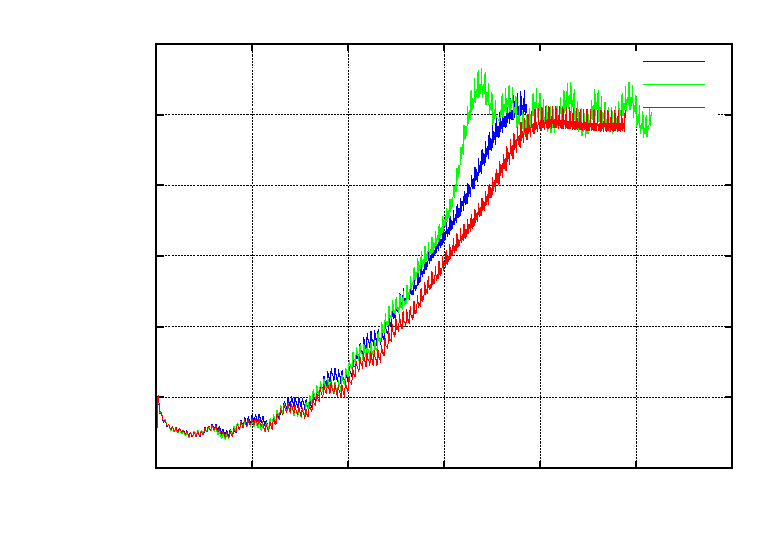
\includegraphics{diskeccentricity}}%
    \gplfronttext
  \end{picture}%
\endgroup

	\end{center}
\end {figure}
\section{Parameterstudie: h, q}
Wir variieren die Parameter Aspectratio H/r, also die Dicke der Disk und den Parameter MassRatio q, das Massenverhältnis des Binärsterns zu dem Primärstern. Ziel ist es, die Wachstumsrate, sowie den Wert der Exzentrizität zu bestimmen. Als Randbedingungen verwenden wir innen reflektierende und aussen offene.
Wir betrachten auch die Präzession der Disk
\subsection{AspectRatio}
\subsection{MassRatio}

\end{document}

